\documentclass[10pt,letterpaper]{article}
\usepackage[top=0.85in,left=2.75in,footskip=0.75in,marginparwidth=2in]{geometry}

% use Unicode characters - try changing the option if you run into troubles with special characters (e.g. umlauts)
\usepackage[utf8]{inputenc}

% clean citations
\usepackage{cite}

% hyperref makes references clicky. use \url{www.example.com} or \href{www.example.com}{description} to add a clicky url
\usepackage{nameref,hyperref}

% line numbers
\usepackage[right]{lineno}

% improves typesetting in LaTeX
\usepackage{microtype}
\DisableLigatures[f]{encoding = *, family = * }

% text layout - change as needed
\raggedright
\setlength{\parindent}{0.5cm}
\textwidth 5.25in 
\textheight 8.75in

% Remove % for double line spacing
%\usepackage{setspace} 
%\doublespacing

% use adjustwidth environment to exceed text width (see examples in text)
\usepackage{changepage}

% adjust caption style
\usepackage[aboveskip=1pt,labelfont=bf,labelsep=period,singlelinecheck=off]{caption}

% remove brackets from references
\makeatletter
\renewcommand{\@biblabel}[1]{\quad#1.}
\makeatother

% headrule, footrule and page numbers
\usepackage{lastpage,fancyhdr,graphicx}
\usepackage{epstopdf}
\pagestyle{myheadings}
\pagestyle{fancy}
\fancyhf{}
\rfoot{\thepage/\pageref{LastPage}}
\renewcommand{\footrule}{\hrule height 2pt \vspace{2mm}}
\fancyheadoffset[L]{2.25in}
\fancyfootoffset[L]{2.25in}

% use \textcolor{color}{text} for colored text (e.g. highlight to-do areas)
\usepackage{color}

% define custom colors (this one is for figure captions)
\definecolor{Gray}{gray}{.25}

% this is required to include graphics
\usepackage{graphicx}

% use if you want to put caption to the side of the figure - see example in text
\usepackage{sidecap}

% use for have text wrap around figures
\usepackage{wrapfig}
\usepackage[pscoord]{eso-pic}
\usepackage[fulladjust]{marginnote}
\reversemarginpar

% document begins here
\begin{document}
\vspace*{0.35in}

% title goes here:
\begin{flushleft}
{\Large
\textbf\newline{\LaTeX Template for Manuscripts with Embedded Figures.}
}
\newline
% authors go here:
\\
Author 1\textsuperscript{1},
Author 2\textsuperscript{2},
Author 3\textsuperscript{1},
Author 4\textsuperscript{1},
Author 5\textsuperscript{2},
Author 6\textsuperscript{2},
Author 7\textsuperscript{1,*}
\\
\bigskip
\bf{1} Affiliation A
\\
\bf{2} Affiliation B
\\
\bigskip
* correseponding@author.mail

\end{flushleft}

\section*{Abstract}
Fitting multiple figures into very tight manuscripts while keeping it pleasant to read is challenging. Therefore figures are often simply attached to the very end of a manuscript file. While easier for the authors, this practice is inconvenient for readers. This \LaTeX template shows how to generate a compiled PDF with figures embedded into the text. It provides several examples of how to embed figures or tables directly into the text thus giving you a range of options from which you should choose the one best suited for your manuscript. Check out Schlegel et al., (2016) as example of use \cite{Schlegel2016}.

% now start line numbers
\linenumbers

% the * after section prevents numbering
\section*{Introduction}
In the introduction you will see an example of text wrapping around the figure with a figure caption on the margin (Fig. \ref{fig1}). This is done by combining the \verb!wrapfigure! with % avoid blank space here 
\marginpar{
\vspace{.7cm} % adjust vertical position relative to text with \vspace{} - note that you can enter negative numbers to move margin caption up
\color{Gray} % this gives caption a grey color to set it apart from text body
\textbf{Figure \ref{fig1}. Example of a margin caption.} % note that \ref{fig1} refers to the corresponding wrapfigure
Setting up your figure + caption like this looks fancy and does not disrupt the flow of the text. But it requires more manual adjustments (position, spacing, labeling) compared to using standard \LaTeX figure environments.
}
\begin{wrapfigure}[19]{l}{75mm}
% the number in [] of wrapfigure is optional and gives the number of text lines that should be wrapped around the text. Adjust according to your figures height
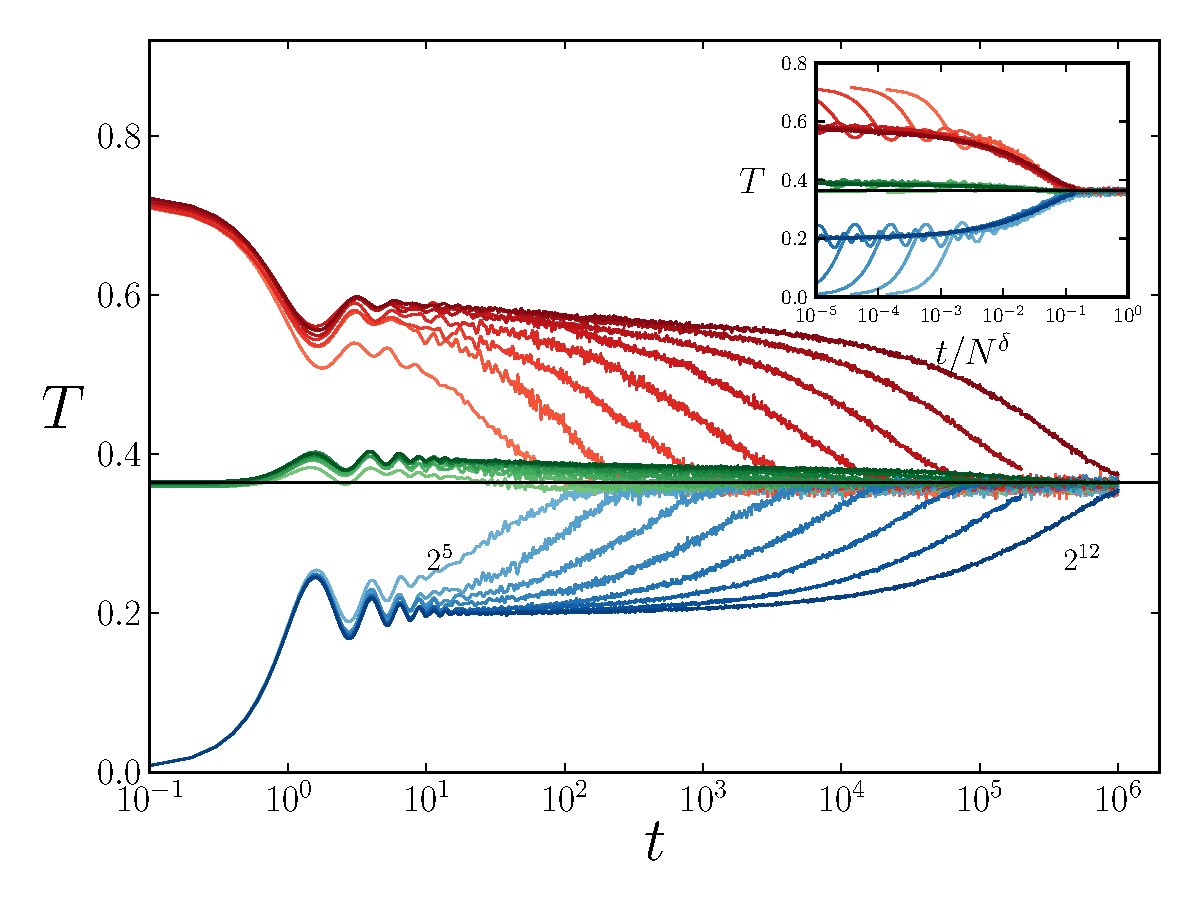
\includegraphics[width=75mm]{figure1.pdf}
\captionsetup{labelformat=empty} % makes sure dummy caption is blank
\caption{} % add dummy caption - otherwise \label won't work and figure numbering will not count up
\label{fig1} % use \ref{fig1} to reference to this figure
\end{wrapfigure} % avoid blank space here
the \verb!marginnote! environment. Please note that in this case the figure (\verb!wrapfigure!) and the figure caption (\verb!marginpar!) have to be separated as you can tell from the code. The \verb!wrapfigure! environment can be a bit tricky when it comes to text formatting. Thus some general hints: (a) try to avoid line breaks in the code as this may result in weird formatting around the figure, (b) the figure should not span multiple headlines (sections) and (c) if you encounter problems with the line break right after the \verb!wrapfigure! try using \verb!\mbox{}! to prevent premature line breaks (\mbox{see example in code}). As stated in the figure caption, setting up figures this way requires a bit more manual adjustments but it makes figures blend in nicely without interrupting flow of text.

\section*{Materials and Methods}

\subsection*{Tables.} 

In this section you will find an example of a table using the \verb!table! plus the \verb!adjustwidth! environment and should give you a minimal example for tables in \LaTeX (Table \ref{tab1}).

\begin{table}[!ht]
\begin{adjustwidth}{-1.5in}{0in} % comment out/remove adjustwidth environment if table fits in text column.
\centering
\caption{{\bf Example Table.} This table demonstrates how to use the  adjustwidth environment if you need that tad bit of extra width for your figures or tables.}
\begin{tabular}{|l|l|l|l|l|l|l|}
\hline
\multicolumn{4}{|l|}{\bf Heading 1} & \multicolumn{3}{|l|}{\bf Heading 2}\\ \hline
cell 1 - row 1 & cell 2 - row 1 & cell 3 - row 1 & cell 4 - row 1 & cell 5 - row 1 & cell 6 - row 1 & cell 7 - row 1 \\ \hline
cell 1 - row 2 & cell 2 - row 2 & cell 3 - row 2 & cell 4 - row 2 & cell 5 - row 2 & cell 6 - row 2 & cell 7 - row 2 \\ \hline
cell 1 - row 3 & cell 2 - row 3 & cell 3 - row 3 & cell 4 - row 3 & cell 5 - row 3 & cell 6 - row 3 & cell 7 - row 3 \\ \hline
\end{tabular}
\label{tab1}
\end{adjustwidth}
\end{table}

\paragraph{Paragraph.}
Instead of adding more and more subsections you can use the \verb!\paragraph{}! command to give structure to your manuscript.

\subsection*{Formulas.}
For mathematical formulas you should use the math environment. See this example:

\begin{center}
$f(A_{ik},A_{jk}) = min(A_{ik},A_{jk}) - C_{1} max(A_{ik},A_{jk}) e^{-C_{2}min(A_{ik},A_{jk})}$
\end{center}

% newpage forces a page break if you want to clearly separate materials from results
\newpage

\section*{Results}
\subsection*{Standard floating figures.}
Figure \ref{fig2} is wrapped into a standard floating environment. That means that \LaTeX will determine the exact placement of the figure. Even though you can state preferences (see code) it can be tricky to get the right placement - especially when working on very tight manuscripts. If you want exact placement, add \verb!\usepackage{float}! to this file's header and use [H] in the figure environment's placement options.


\begin{figure}[ht] %s state preferences regarding figure placement here

% use to correct figure counter if necessary
%\renewcommand{\thefigure}{2}

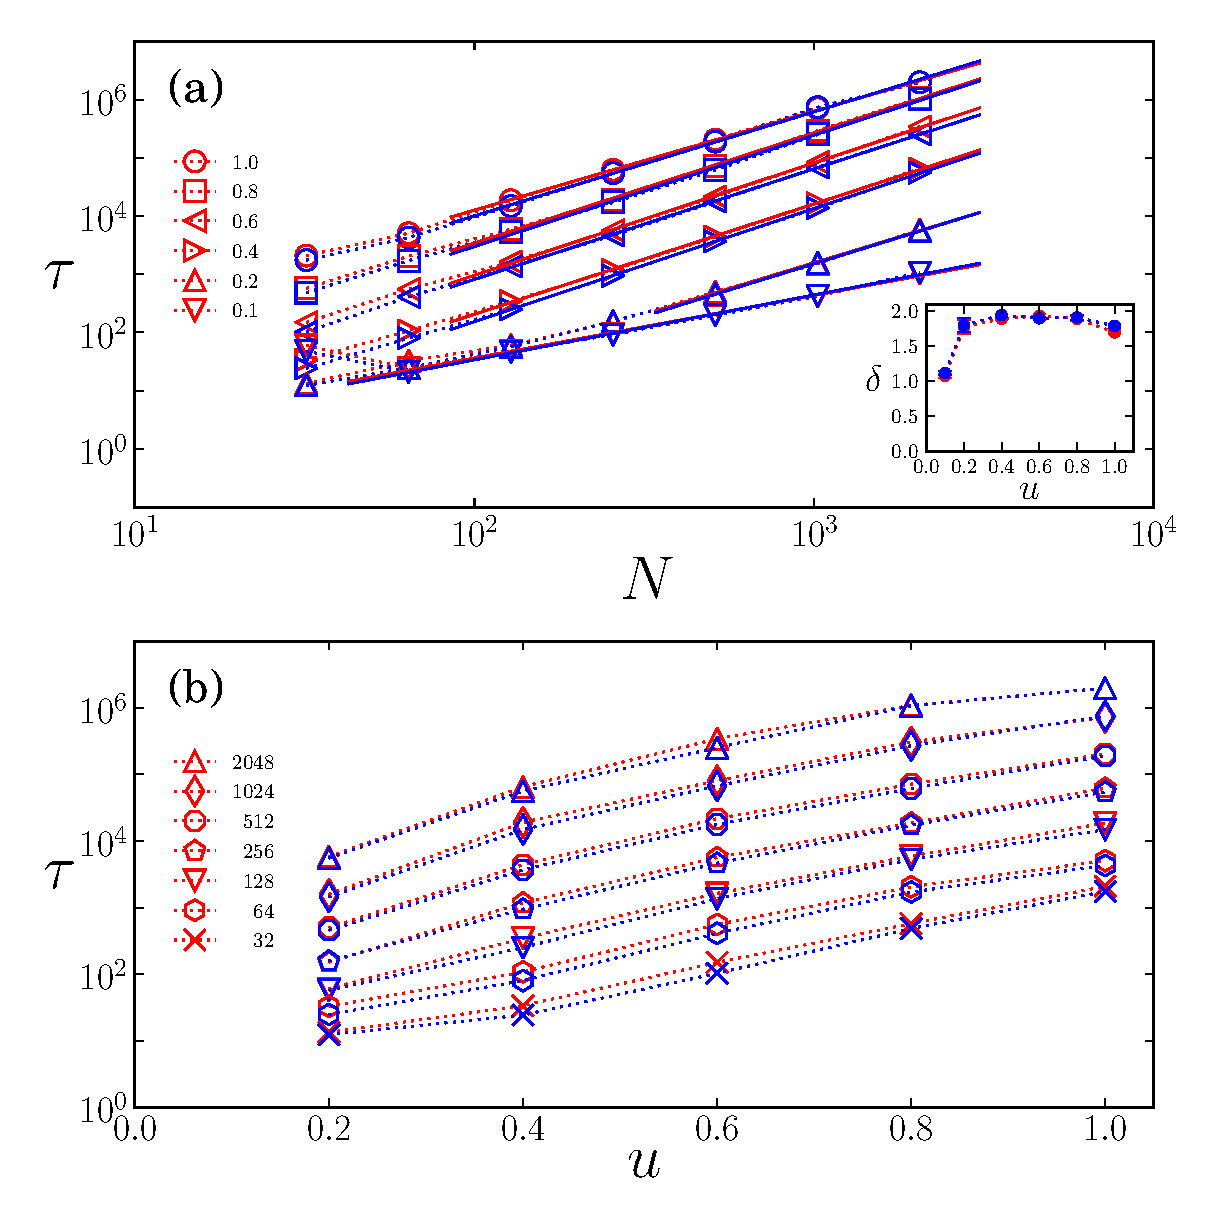
\includegraphics[width=\textwidth]{figure2.pdf}

\caption{\color{Gray} \textbf{Example of a standard floating figure}. \textbf{A-F}, This figure is wrapped into the standard floating environment.}

\label{fig2} % \label works only AFTER \caption within figure environment

\end{figure}

\subsection*{Page break in figures.}
The standard floating figures in \LaTeX do not cope well with page breaks which can make it difficult to fit in large figures. One way to deal with this is to separate figure and caption but \verb!\caption{}! might still give troubles at page breaks. Figure 3 demonstrates a way to manually set up figure and caption such that it continues onto the next page.
\vspace{.5cm} % set vertical space between text and figure
\begin{adjustwidth}{-2in}{0in}
\begin{flushright}
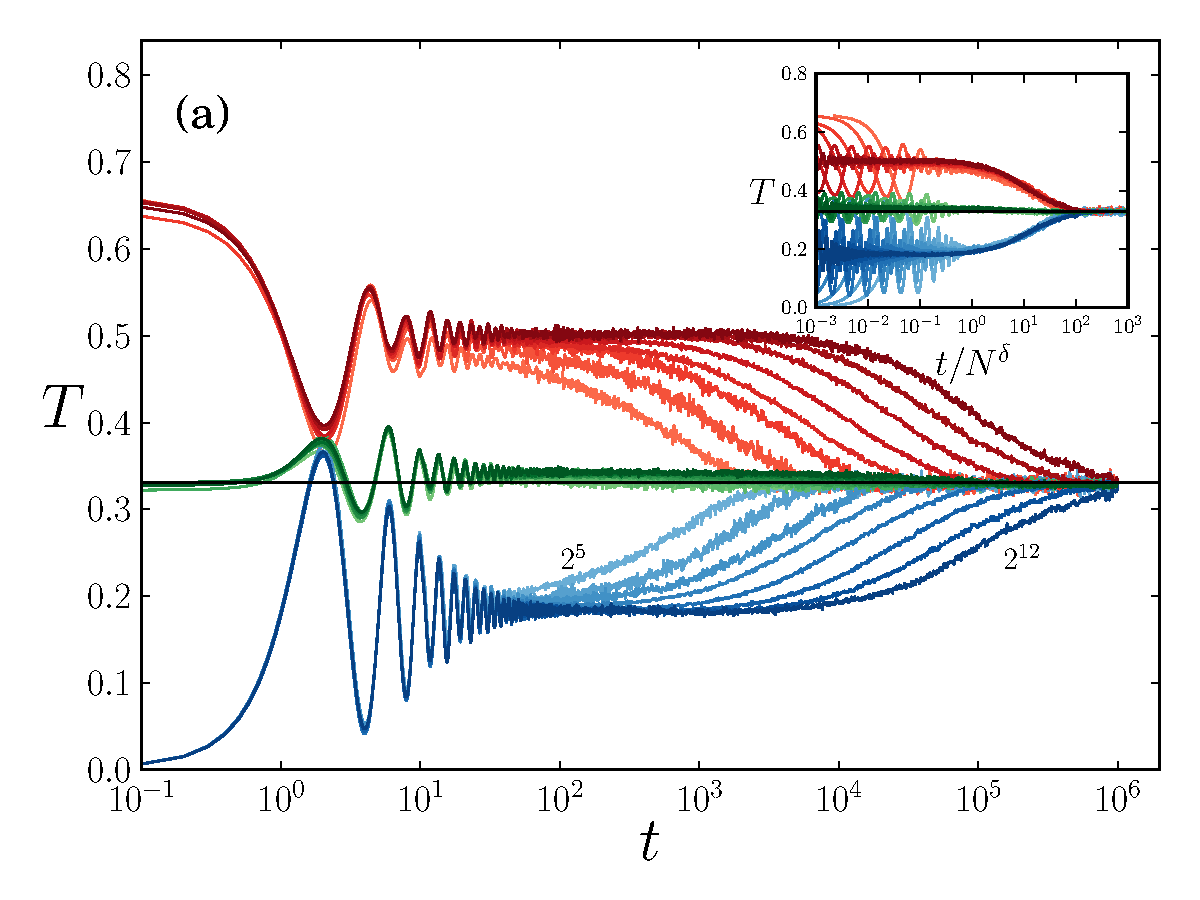
\includegraphics[width=163mm]{figure3a.pdf}
\end{flushright}
\justify 
\color{Gray}
\textbf {Figure 3. Example of a wide figure with multi-page caption.}
\textbf{A}, Proin lectus ex, venenatis vel ornare eget, hendrerit tempus justo. Pellentesque molestie purus sed pretium tincidunt. Curabitur facilisis, orci vitae mollis fringilla, elit erat fermentum justo, nec luctus nunc sapien vel dolor. Cras enim justo, ullamcorper ut commodo at, posuere et ex. Fusce cursus sapien id augue maximus convallis. Praesent egestas massa in enim volutpat varius. In aliquam turpis urna, at elementum turpis eleifend at. \textbf{B}, Proin risus erat, tincidunt quis massa non, sollicitudin congue metus. Aliquam quis magna vulputate, posuere est eu, tempor nisi. Cras gravida tempus felis, vitae lacinia lacus volutpat quis. Pellentesque et eros eu mi suscipit tempus. Proin in augue scelerisque. \textbf{C}, Donec a tempor tortor, et dignissim enim. Cras in ipsum sed velit bibendum imperdiet. Aenean aliquet mauris maximus, sodales ligula sit amet, placerat felis. In tristique nisi eu risus rutrum, ac lacinia lorem cursus. Nunc eget condimentum purus. Maecenas imperdiet nisl eu accumsan gravida. \textbf{D}, Nullam tincidunt, magna sed auctor ultrices, leo mi eleifend velit, quis varius ex diam non tellus. Nam tincidunt vehicula turpis, ut euismod turpis elementum vel.
\end{adjustwidth}


%\clearpage makes sure that all above content is printed at this point and does not invade into the upcoming content
%\clearpage

\section*{Discussion}
\subsection*{Subsection heading.}

Lorem ipsum dolor sit amet, consectetur adipiscing elit. Aliquam bibendum finibus diam, gravida sagittis lorem gravida vitae. Interdum et malesuada fames ac ante ipsum primis in faucibus. Nulla in diam tristique ante posuere tristique. Donec interdum purus sit amet nisl accumsan consectetur. Fusce aliquet libero mi, quis ornare dolor congue ullamcorper. Nulla nulla urna, molestie in urna sed, lacinia volutpat eros. Ut mi libero, elementum scelerisque ipsum vel, hendrerit fermentum turpis. Aliquam sit amet leo sodales, egestas augue id, fermentum nulla. Aenean vel cursus ante, et pellentesque eros. Nulla ac neque nec justo posuere commodo sit amet sit amet justo. Aliquam tincidunt tempor ex nec tincidunt. In ullamcorper vehicula lobortis. 

%\clearpage

\section*{Supporting Information}
If you intend to keep supporting files separately you can do so and just provide figure captions here. Optionally make clicky links to the online file using \verb!\href{url}{description}!.

%These commands reset the figure counter and add "S" to the figure caption (e.g. "Figure S1"). This is in case you want to add actual figures and not just captions.
\setcounter{figure}{0}
\renewcommand{\thefigure}{S\arabic{figure}}

% You can use the \nameref{label} command to cite supporting items in the text.
\subsection*{S1 Figure}
\label{example_label}
{\bf Caption of Figure S1.} \textbf{A}, If you want to reference supporting figures in the text, use the \verb!\nameref{}!. command. This will reference the section's heading: \nameref{example_label}.

\subsection*{S2 Video}
\label{example_video}
{\bf Example Video.} Use \href{www.youtube.com}{clicky links} to the online sources of the files.

%\clearpage

\section*{Acknowledgments}
We thank just about everybody.

\nolinenumbers

%This is where your bibliography is generated. Make sure that your .bib file is actually called library.bib
%\bibliography{library}

%This defines the bibliographies style. Search online for a list of available styles.
%\bibliographystyle{abbrv}

\end{document}



